% -*- TeX-engine: luatex -*-
\documentclass[presentation,aspectratio=43, 10pt]{beamer}
\usepackage{pifont}
\newcommand{\cmark}{\ding{51}}
\newcommand{\xmark}{\ding{55}}

\usepackage{booktabs}
\titlegraphic{\hfill
\includegraphics[height=1.25cm]{durham-logo}}
\usepackage{appendixnumberbeamer}
\usepackage{amsmath}
\usepackage{amssymb}
\usepackage{mathtools}
\usepackage{hyperref}
\usepackage{xspace}
\newcommand{\arxivlink}[2]{{\texttt{arXiv:\,\href{https://arxiv.org/abs/#1}{#1\,[#2]}}}}

\newcommand{\honev}{\ensuremath{{H}^1(\Omega; \mathbb{R}^d)}\xspace}
\newcommand{\ltwov}{\ensuremath{{L}^2(\Omega; \mathbb{R}^d)}\xspace}
\newcommand{\ltwo}{\ensuremath{{L}^2(\Omega)}\xspace}
\newcommand{\inner}[1]{\left\langle #1 \right \rangle}
\DeclareMathOperator{\Adj}{Adj}

\usepackage{pgfplots}
\usepackage{pgfplotstable}
\usepgfplotslibrary{dateplot}
\usepackage{minted}
\usepackage[url=false,
doi=true,
isbn=false,
style=authoryear,
maxnames=5,
giveninits=true,
uniquename=init,
backend=biber]{biblatex}
\renewcommand{\bibfont}{\fontsize{7}{7}\selectfont}
\addbibresource{../literature.bib}

\setlength{\bibitemsep}{1ex}
\setlength{\fboxsep}{1pt}

\renewbibmacro{in:}{}
\DeclareFieldFormat[article]{volume}{\textbf{#1}}
\DeclareFieldFormat{doi}{%
  doi\addcolon%
  {\scriptsize\ifhyperref{\href{http://dx.doi.org/#1}{\nolinkurl{#1}}}
    {\nolinkurl{#1}}}}
\AtEveryBibitem{%
\clearfield{pages}%
\clearfield{issue}%
\clearfield{number}%
}

\DeclareMathOperator{\grad}{grad}
\let\div\relax
\DeclareMathOperator{\div}{div}
\DeclareMathOperator{\curl}{curl}
\DeclareMathOperator{\range}{range}
\DeclareMathOperator{\sym}{sym}
\usetheme{metropolis}
\setbeamertemplate{title graphic}{
  \vbox to 0pt {
    \vspace*{1em}
    \inserttitlegraphic%
  }%
  \nointerlineskip%
}
\metroset{background=light,progressbar=frametitle,numbering=counter,block=fill}

% https://www.dur.ac.uk/marketingandcommunications/marketing/branding/colourpalette/
% Most of these are indistinguishable to those suffering colour blindness
\definecolor{purple}{HTML}{68246D}
\definecolor{blue}{HTML}{002A41}
\definecolor{red}{HTML}{BE1E2D}
\definecolor{cyan}{HTML}{00AEEF}
\definecolor{yellow}{HTML}{FFD53A}

\setbeamercolor{normal text}{
  fg=black,
  bg=white
}
\setbeamercolor{alerted text}{
  fg=red
}
\setbeamercolor{example text}{
  fg=blue
}

\setbeamercolor{palette primary}{%
  use=normal text,
  fg=normal text.bg,
  bg=purple,
}

\usetheme{metropolis}

\author{Lawrence Mitchell}
\institute{
  Department of Computer Science, Durham University\\
  \texttt{lawrence.mitchell@durham.ac.uk}}

\title{Representing structure in computational meshes}

\usepackage{tikz}
\usetikzlibrary{trees,calc,positioning}
\usetikzlibrary{shapes, shapes.geometric}
\usetikzlibrary{arrows,chains,positioning,fit,backgrounds,calc,shapes,
  shadows,scopes,decorations.markings,plotmarks}

\newcommand*{\tettextsize}{\footnotesize}
\tikzstyle{line} = [draw, -, thick]
\tikzstyle{nodraw} = [draw, fill, circle, minimum width=0pt, inner sep=0pt]
\tikzstyle{sieve} = [line, circle, font=\tettextsize, inner sep=0pt,
  minimum size=12pt]

\tikzstyle{cell} = [sieve, fill=blue!60]
\tikzstyle{facet} = [sieve, fill=green!35]
\tikzstyle{edge} = [sieve, fill=red!35]
\tikzstyle{vertex} = [sieve, fill=blue!35]

% https://tex.stackexchange.com/questions/27171/padded-boundary-of-convex-hull
\newcommand{\convexpath}[2]{
  [
  create hullcoords/.code={
    \global\edef\namelist{#1}
    \foreach [count=\counter] \nodename in \namelist {
      \global\edef\numberofnodes{\counter}
      \coordinate (hullcoord\counter) at (\nodename);
    }
    \coordinate (hullcoord0) at (hullcoord\numberofnodes);
    \pgfmathtruncatemacro\lastnumber{\numberofnodes+1}
    \coordinate (hullcoord\lastnumber) at (hullcoord1);
  },
  create hullcoords
  ]
  ($(hullcoord1)!#2!-90:(hullcoord0)$)
  \foreach [
  evaluate=\currentnode as \previousnode using \currentnode-1,
  evaluate=\currentnode as \nextnode using \currentnode+1
  ] \currentnode in {1,...,\numberofnodes} {
    let \p1 = ($(hullcoord\currentnode) - (hullcoord\previousnode)$),
    \n1 = {atan2(\y1,\x1) + 90},
    \p2 = ($(hullcoord\nextnode) - (hullcoord\currentnode)$),
    \n2 = {atan2(\y2,\x2) + 90},
    \n{delta} = {Mod(\n2-\n1,360) - 360}
    in
    {arc [start angle=\n1, delta angle=\n{delta}, radius=#2]}
    -- ($(hullcoord\nextnode)!#2!-90:(hullcoord\currentnode)$)
  }
}

\graphicspath{{./\jobname.figures/}{../pictures/}}
\date{10 March 2020}
\begin{document}

\maketitle

% \begin{abstract}
%   Many mesh-based simulations occur on meshes with some regular
%   structure. Examples include, but are not limited to: composite
%   macro-elements and high continuity spline discretisations; regular
%   refinement in geometric multigrid; structured mesh extrusion (common
%   in ocean, ice sheet, and atmospheric modelling); and octree-like
%   AMR.

%   An unanswered question is how to handle these and other kinds of
%   structure in meshes in a composable way. For example, what if I want
%   a macro-element on an extruded mesh must I program that case by hand?

%   I presented the way in which we (in the Firedrake project)
%   represent unstructured meshes and provided some nascent musing on
%   symbolic interfaces for code generators that might exploit some
%   structure. A particular focus was maintaining the ability to
%   perform topological queries of the "symbolic" meshes.
% \end{abstract}


\begin{frame}[fragile]
  \frametitle{Typical mesh-based code}
  \begin{block}{Residual evaluation}
\begin{minted}[fontsize=\scriptsize]{python}
  ulocal <- global_to_local(uglobal)
  foreach element in mesh:
      uelement <- local_to_element(ulocal)
      relement <- compute_on_local(uelement)
      rlocal <- element_to_local(relement)
  rglobal <- local_to_global(rlocal)
\end{minted}
  \end{block}
  \begin{itemize}
  \item Cannot avoid moving field data
  \item \verb|local_to_element| uses topology of mesh (element->dof
    map)
  \item Can I avoid moving data for this?
  \end{itemize}
\end{frame}

\begin{frame}
  \frametitle{Abstract representation of meshes}
  \begin{itemize}
  \item As a graph with restrictions on the structure
  \item Idea: every geometric entity in mesh $\Rightarrow$ vertex in
    graph;
  \item Relationship between entities (e.g. edges of a face)
    $\Rightarrow$ edge in graph.
  \item For conforming meshes, this is graph is bipartite.
  \item Can also use ideas from algebraic topology, e.g.~\textcite{Knepley:2009}
    \arxivlink{0908.4427}{cs.CE}, to formalise lots of the
    operations.
  \end{itemize}
\end{frame}
\begin{frame}[t]
  \frametitle{DMPlex/Sieve notation, data structures}
  \begin{columns}[T]
    \begin{column}{0.4\textwidth}
      \begin{block}{Mesh}
        \begin{center}
          \begin{tikzpicture}
            \node (0) [nodraw, label=below:{\tettextsize 2}] at (0,0) {};
\node (1) [nodraw, label=below:{\tettextsize 3}] at (2.4,0) {};
\node (2) [nodraw, label=above right:{\tettextsize 4}] at (2.3,0.84) {};
\node (3) [nodraw, label=above:{\tettextsize 1}] at (1.2,2.0) {};

\path[line] (0) edge node[label=below:{\tettextsize 9}]{} (1);
%% \draw[line] (0) -- (1);
\path[line, dashed] (0) edge node[label=above:{\tettextsize 14}]{} (2);
\path[line] (1) edge node[label=right:{\tettextsize 12}]{} (2);
\draw[line] (0) edge node[label=above left:{\tettextsize 11}]{} (3);
\draw[line] (1) edge node[label=left:{\tettextsize 10}]{} (3);
\draw[line] (2) edge node[label=above right:{\tettextsize 13}]{} (3);

          \end{tikzpicture}
        \end{center}
        Vertices, edges, and cell labelled.
      \end{block}
    \end{column}
    \begin{column}{0.6\textwidth}
      \begin{block}{Graph representation}
        \begin{onlyenv}<1>
          \begin{center}
            \begin{tikzpicture}
              \def\y{.79}
\def\x{.32}
\node (0) [cell] at (0,0) {0};
\node (1) [facet] at (-3*\x, \y) {5};
\node (2) [facet] at (-1*\x, \y) {6};
\node (3) [facet] at (1*\x, \y) {7};
\node (4) [facet] at (3*\x, \y) {8};
\node (5) [edge] at (-4*\x, 2*\y) {9};
\node (6) [edge] at (-2.4*\x, 2*\y) {10};
\node (7) [edge] at (-.8*\x, 2*\y) {11};
\node (8) [edge] at (.8*\x, 2*\y) {12};
\node (9) [edge] at (2.4*\x, 2*\y) {13};
\node (10) [edge] at (4*\x, 2*\y) {14};
\node (11) [vertex] at (-3*\x, 3*\y) {1};
\node (12) [vertex] at (-1*\x, 3*\y) {2};
\node (13) [vertex] at (1*\x, 3*\y) {3};
\node (14) [vertex] at (3*\x, 3*\y) {4};

\draw[line] (0) -- (1);
\draw[line] (0) -- (2);
\draw[line] (0) -- (3);
\draw[line] (0) -- (4);
\draw[line] (1) -- (5);
\draw[line] (1) -- (6);
\draw[line] (1) -- (7);
\draw[line] (2) -- (6);
\draw[line] (2) -- (8);
\draw[line] (2) -- (9);
\draw[line] (3) -- (7);
\draw[line] (3) -- (9);
\draw[line] (3) -- (10);
\draw[line] (4.north west) -- (5.south east);
\draw[line] (4) -- (8);
\draw[line] (4) -- (10);
\draw[line] (5) -- (12);
\draw[line] (5) -- (13);
\draw[line] (6) -- (11);
\draw[line] (6) -- (13);
\draw[line] (7) -- (11);
\draw[line] (7) -- (12);
\draw[line] (8) -- (13);
\draw[line] (8) -- (14);
\draw[line] (9) -- (11);
\draw[line] (9) -- (14);
\draw[line] (10) -- (12);
\draw[line] (10) -- (14);

            \end{tikzpicture}
          \end{center}
        \end{onlyenv}
        \begin{onlyenv}<2>
          \begin{center}
            \begin{tikzpicture}
              \def\y{.79}
\def\x{.32}
\node (0) [cell] at (0,0) {0};
\node (1) [facet] at (-3*\x, \y) {5};
\node (2) [facet] at (-1*\x, \y) {6};
\node (3) [facet] at (1*\x, \y) {7};
\node (4) [facet] at (3*\x, \y) {8};
\node (5) [edge] at (-4*\x, 2*\y) {9};
\node (6) [edge] at (-2.4*\x, 2*\y) {10};
\node (7) [edge] at (-.8*\x, 2*\y) {11};
\node (8) [edge] at (.8*\x, 2*\y) {12};
\node (9) [edge] at (2.4*\x, 2*\y) {13};
\node (10) [edge] at (4*\x, 2*\y) {14};
\node (11) [vertex] at (-3*\x, 3*\y) {1};
\node (12) [vertex] at (-1*\x, 3*\y) {2};
\node (13) [vertex] at (1*\x, 3*\y) {3};
\node (14) [vertex] at (3*\x, 3*\y) {4};

\draw[line] (0) -- (1);
\draw[line] (0) -- (2);
\draw[line] (0) -- (3);
\draw[line] (0) -- (4);
\draw[line] (1) -- (5);
\draw[line] (1) -- (6);
\draw[line] (1) -- (7);
\draw[line] (2) -- (6);
\draw[line] (2) -- (8);
\draw[line] (2) -- (9);
\draw[line] (3) -- (7);
\draw[line] (3) -- (9);
\draw[line] (3) -- (10);
\draw[line] (4.north west) -- (5.south east);
\draw[line] (4) -- (8);
\draw[line] (4) -- (10);
\draw[line] (5) -- (12);
\draw[line] (5) -- (13);
\draw[line] (6) -- (11);
\draw[line] (6) -- (13);
\draw[line] (7) -- (11);
\draw[line] (7) -- (12);
\draw[line] (8) -- (13);
\draw[line] (8) -- (14);
\draw[line] (9) -- (11);
\draw[line] (9) -- (14);
\draw[line] (10) -- (12);
\draw[line] (10) -- (14);

              \begin{scope}[overlay, remember picture, rounded corners]
                \filldraw[fill opacity=0.2]
                ([xshift= 3pt, yshift=-3pt] 7.south east) --
                ([xshift= 3pt, yshift= 3pt] 7.north east) --
                ([xshift=-3pt, yshift= 3pt] 5.north west) --
                ([xshift=-3pt, yshift=-3pt] 5.south west) --
                cycle;
                \node[cell, fill=black, opacity=0.6] at (1.center) {};
              \end{scope}
            \end{tikzpicture}
          \end{center}
          $\text{\texttt{cone}}(5) = \{9, 10, 11\}$
        \end{onlyenv}
        \begin{onlyenv}<3>
          \begin{center}
            \begin{tikzpicture}
              \def\y{.79}
\def\x{.32}
\node (0) [cell] at (0,0) {0};
\node (1) [facet] at (-3*\x, \y) {5};
\node (2) [facet] at (-1*\x, \y) {6};
\node (3) [facet] at (1*\x, \y) {7};
\node (4) [facet] at (3*\x, \y) {8};
\node (5) [edge] at (-4*\x, 2*\y) {9};
\node (6) [edge] at (-2.4*\x, 2*\y) {10};
\node (7) [edge] at (-.8*\x, 2*\y) {11};
\node (8) [edge] at (.8*\x, 2*\y) {12};
\node (9) [edge] at (2.4*\x, 2*\y) {13};
\node (10) [edge] at (4*\x, 2*\y) {14};
\node (11) [vertex] at (-3*\x, 3*\y) {1};
\node (12) [vertex] at (-1*\x, 3*\y) {2};
\node (13) [vertex] at (1*\x, 3*\y) {3};
\node (14) [vertex] at (3*\x, 3*\y) {4};

\draw[line] (0) -- (1);
\draw[line] (0) -- (2);
\draw[line] (0) -- (3);
\draw[line] (0) -- (4);
\draw[line] (1) -- (5);
\draw[line] (1) -- (6);
\draw[line] (1) -- (7);
\draw[line] (2) -- (6);
\draw[line] (2) -- (8);
\draw[line] (2) -- (9);
\draw[line] (3) -- (7);
\draw[line] (3) -- (9);
\draw[line] (3) -- (10);
\draw[line] (4.north west) -- (5.south east);
\draw[line] (4) -- (8);
\draw[line] (4) -- (10);
\draw[line] (5) -- (12);
\draw[line] (5) -- (13);
\draw[line] (6) -- (11);
\draw[line] (6) -- (13);
\draw[line] (7) -- (11);
\draw[line] (7) -- (12);
\draw[line] (8) -- (13);
\draw[line] (8) -- (14);
\draw[line] (9) -- (11);
\draw[line] (9) -- (14);
\draw[line] (10) -- (12);
\draw[line] (10) -- (14);

              \begin{scope}[overlay, remember picture, rounded corners]
                \filldraw[fill opacity=0.2]
                ([xshift= 1pt, yshift=-3pt] 1.south east) --
                ([xshift=-3pt, yshift= 1pt] 2.north west) --
                ([xshift= 3pt, yshift=-1pt] 7.south east) --
                ([xshift=-3pt, yshift= 1pt] 8.north west) --
                ([xshift= 3pt, yshift=-1pt] 13.south east) --
                ([xshift= 3pt, yshift= 3pt] 13.north east) --
                ([xshift=-2pt, yshift= 3pt] 11.north west) --
                ([xshift=-2pt, yshift= 0pt] 5.west) --
                ([xshift=-1pt, yshift=-3pt] 1.south west) --
                cycle;
                \node[cell, fill=black, opacity=0.6] at (1.center) {};
              \end{scope}
            \end{tikzpicture}
          \end{center}
          $\text{\texttt{closure}}(5) = \{1, 2, 3, 9, 10, 11, 5\}$
        \end{onlyenv}
        \begin{onlyenv}<4>
          \begin{center}
            \begin{tikzpicture}
              \def\y{.79}
\def\x{.32}
\node (0) [cell] at (0,0) {0};
\node (1) [facet] at (-3*\x, \y) {5};
\node (2) [facet] at (-1*\x, \y) {6};
\node (3) [facet] at (1*\x, \y) {7};
\node (4) [facet] at (3*\x, \y) {8};
\node (5) [edge] at (-4*\x, 2*\y) {9};
\node (6) [edge] at (-2.4*\x, 2*\y) {10};
\node (7) [edge] at (-.8*\x, 2*\y) {11};
\node (8) [edge] at (.8*\x, 2*\y) {12};
\node (9) [edge] at (2.4*\x, 2*\y) {13};
\node (10) [edge] at (4*\x, 2*\y) {14};
\node (11) [vertex] at (-3*\x, 3*\y) {1};
\node (12) [vertex] at (-1*\x, 3*\y) {2};
\node (13) [vertex] at (1*\x, 3*\y) {3};
\node (14) [vertex] at (3*\x, 3*\y) {4};

\draw[line] (0) -- (1);
\draw[line] (0) -- (2);
\draw[line] (0) -- (3);
\draw[line] (0) -- (4);
\draw[line] (1) -- (5);
\draw[line] (1) -- (6);
\draw[line] (1) -- (7);
\draw[line] (2) -- (6);
\draw[line] (2) -- (8);
\draw[line] (2) -- (9);
\draw[line] (3) -- (7);
\draw[line] (3) -- (9);
\draw[line] (3) -- (10);
\draw[line] (4.north west) -- (5.south east);
\draw[line] (4) -- (8);
\draw[line] (4) -- (10);
\draw[line] (5) -- (12);
\draw[line] (5) -- (13);
\draw[line] (6) -- (11);
\draw[line] (6) -- (13);
\draw[line] (7) -- (11);
\draw[line] (7) -- (12);
\draw[line] (8) -- (13);
\draw[line] (8) -- (14);
\draw[line] (9) -- (11);
\draw[line] (9) -- (14);
\draw[line] (10) -- (12);
\draw[line] (10) -- (14);

              \begin{scope}[overlay, remember picture, rounded corners]
                \filldraw[fill opacity=0.2]
                ([xshift= 3pt, yshift=-3pt] 10.south east) --
                ([xshift= 3pt, yshift= 3pt] 10.north east) --
                ([xshift=-3pt, yshift= 3pt] 8.north west) --
                ([xshift=-3pt, yshift=-3pt] 8.south west) --
                cycle;
                \node[cell, fill=black, opacity=0.6] at (14.center) {};
              \end{scope}
            \end{tikzpicture}
          \end{center}
          $\text{\texttt{support}}(4) = \{12, 13, 14\}$
        \end{onlyenv}
        \begin{onlyenv}<5>
          \begin{center}
            \begin{tikzpicture}
              \def\y{.79}
\def\x{.32}
\node (0) [cell] at (0,0) {0};
\node (1) [facet] at (-3*\x, \y) {5};
\node (2) [facet] at (-1*\x, \y) {6};
\node (3) [facet] at (1*\x, \y) {7};
\node (4) [facet] at (3*\x, \y) {8};
\node (5) [edge] at (-4*\x, 2*\y) {9};
\node (6) [edge] at (-2.4*\x, 2*\y) {10};
\node (7) [edge] at (-.8*\x, 2*\y) {11};
\node (8) [edge] at (.8*\x, 2*\y) {12};
\node (9) [edge] at (2.4*\x, 2*\y) {13};
\node (10) [edge] at (4*\x, 2*\y) {14};
\node (11) [vertex] at (-3*\x, 3*\y) {1};
\node (12) [vertex] at (-1*\x, 3*\y) {2};
\node (13) [vertex] at (1*\x, 3*\y) {3};
\node (14) [vertex] at (3*\x, 3*\y) {4};

\draw[line] (0) -- (1);
\draw[line] (0) -- (2);
\draw[line] (0) -- (3);
\draw[line] (0) -- (4);
\draw[line] (1) -- (5);
\draw[line] (1) -- (6);
\draw[line] (1) -- (7);
\draw[line] (2) -- (6);
\draw[line] (2) -- (8);
\draw[line] (2) -- (9);
\draw[line] (3) -- (7);
\draw[line] (3) -- (9);
\draw[line] (3) -- (10);
\draw[line] (4.north west) -- (5.south east);
\draw[line] (4) -- (8);
\draw[line] (4) -- (10);
\draw[line] (5) -- (12);
\draw[line] (5) -- (13);
\draw[line] (6) -- (11);
\draw[line] (6) -- (13);
\draw[line] (7) -- (11);
\draw[line] (7) -- (12);
\draw[line] (8) -- (13);
\draw[line] (8) -- (14);
\draw[line] (9) -- (11);
\draw[line] (9) -- (14);
\draw[line] (10) -- (12);
\draw[line] (10) -- (14);
 
              \begin{scope}[overlay, remember picture, rounded corners]
                \filldraw[fill opacity=0.2]
                ([xshift= 0pt, yshift= 3pt] 14.north west) --
                ([xshift= 3pt, yshift=-3pt] 13.south east) --
                ([xshift=-3pt, yshift= 1pt] 8.north west) --
                ([xshift= 3pt, yshift=-1pt] 7.south east) --
                ([xshift=-3pt, yshift= 1pt] 2.north west) --
                ([xshift=-3pt, yshift= 1pt] 2.south west) --
                ([xshift= 0pt, yshift=-3pt] 0.south west) --
                ([xshift= 0pt, yshift=-3pt] 0.south east) --
                ([xshift= 3pt, yshift=-1pt] 4.south east) --
                ([xshift= 3pt, yshift= 0pt] 10.east) --
                ([xshift= 2pt, yshift= 3pt] 14.north east) --
                cycle;
                \node[cell, fill=black, opacity=0.6] at (14.center) {};
              \end{scope}
            \end{tikzpicture}
          \end{center}
          $\text{\texttt{star}}(4) = \{0, 6, 7, 8, 12, 13, 14, 4\}$
        \end{onlyenv}
      \end{block}
    \end{column}
  \end{columns}
\end{frame}



\begin{frame}
  \frametitle{Topological queries}
  \begin{itemize}
  \item This setup permits dimension-independent code for querying
    topological relationships in the mesh
  \item Can do all the normal things for finite element assembly: grab
    all data associated with a single cell.
  \end{itemize}

  \begin{block}{Challenge: structure}
    \begin{itemize}
    \item Implementation assumes fully unstructured.
    \item Can this same idea be extended to meshes that offer some
      structure
    \item \dots while exploiting that structure for a fast implementation?
    \end{itemize}
  \end{block}
\end{frame}

\begin{frame}
  \frametitle{Idea: exploit structure}
  \begin{definition}[Unstructured mesh $\mathbb{U}$]
    Relationship between mesh entities provided by explicit
    enumeration.

    $\Rightarrow$ need to store relationship in arrays: data movement.
  \end{definition}
  \begin{definition}[Semi-structured mesh $\mathbb{U} \otimes \mathbb{S}$]
    Relationship between mesh entities sometimes available through
    closed form expression.
  \end{definition}
  \begin{definition}[Structured mesh $\mathbb{S}$]
    Relationship between mesh entities provided by closed form
    arithmetic expression

    $\Rightarrow$ less data movement
  \end{definition}
\end{frame}
\begin{frame}
  \frametitle{Examples}
  \begin{overlayarea}{\textwidth}{0.9\textheight}
    \begin{onlyenv}<1>
      \begin{block}{Extruded meshes}
        Often used in atmosphere, ocean, and ice sheet modelling. One
        structured direction.

        \begin{center}
          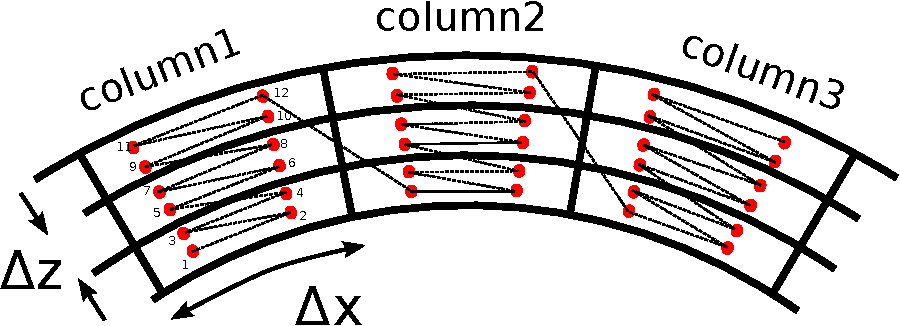
\includegraphics[height=0.4\textheight]{columndofs}
        \end{center}
      \end{block}
    \end{onlyenv}
    \begin{onlyenv}<2>
      \begin{block}{Barycentric refinement}
        Used for stability for Scott-Vogelius element pair,
        macro-element construction for $C^1$ elements.
        \begin{center}
          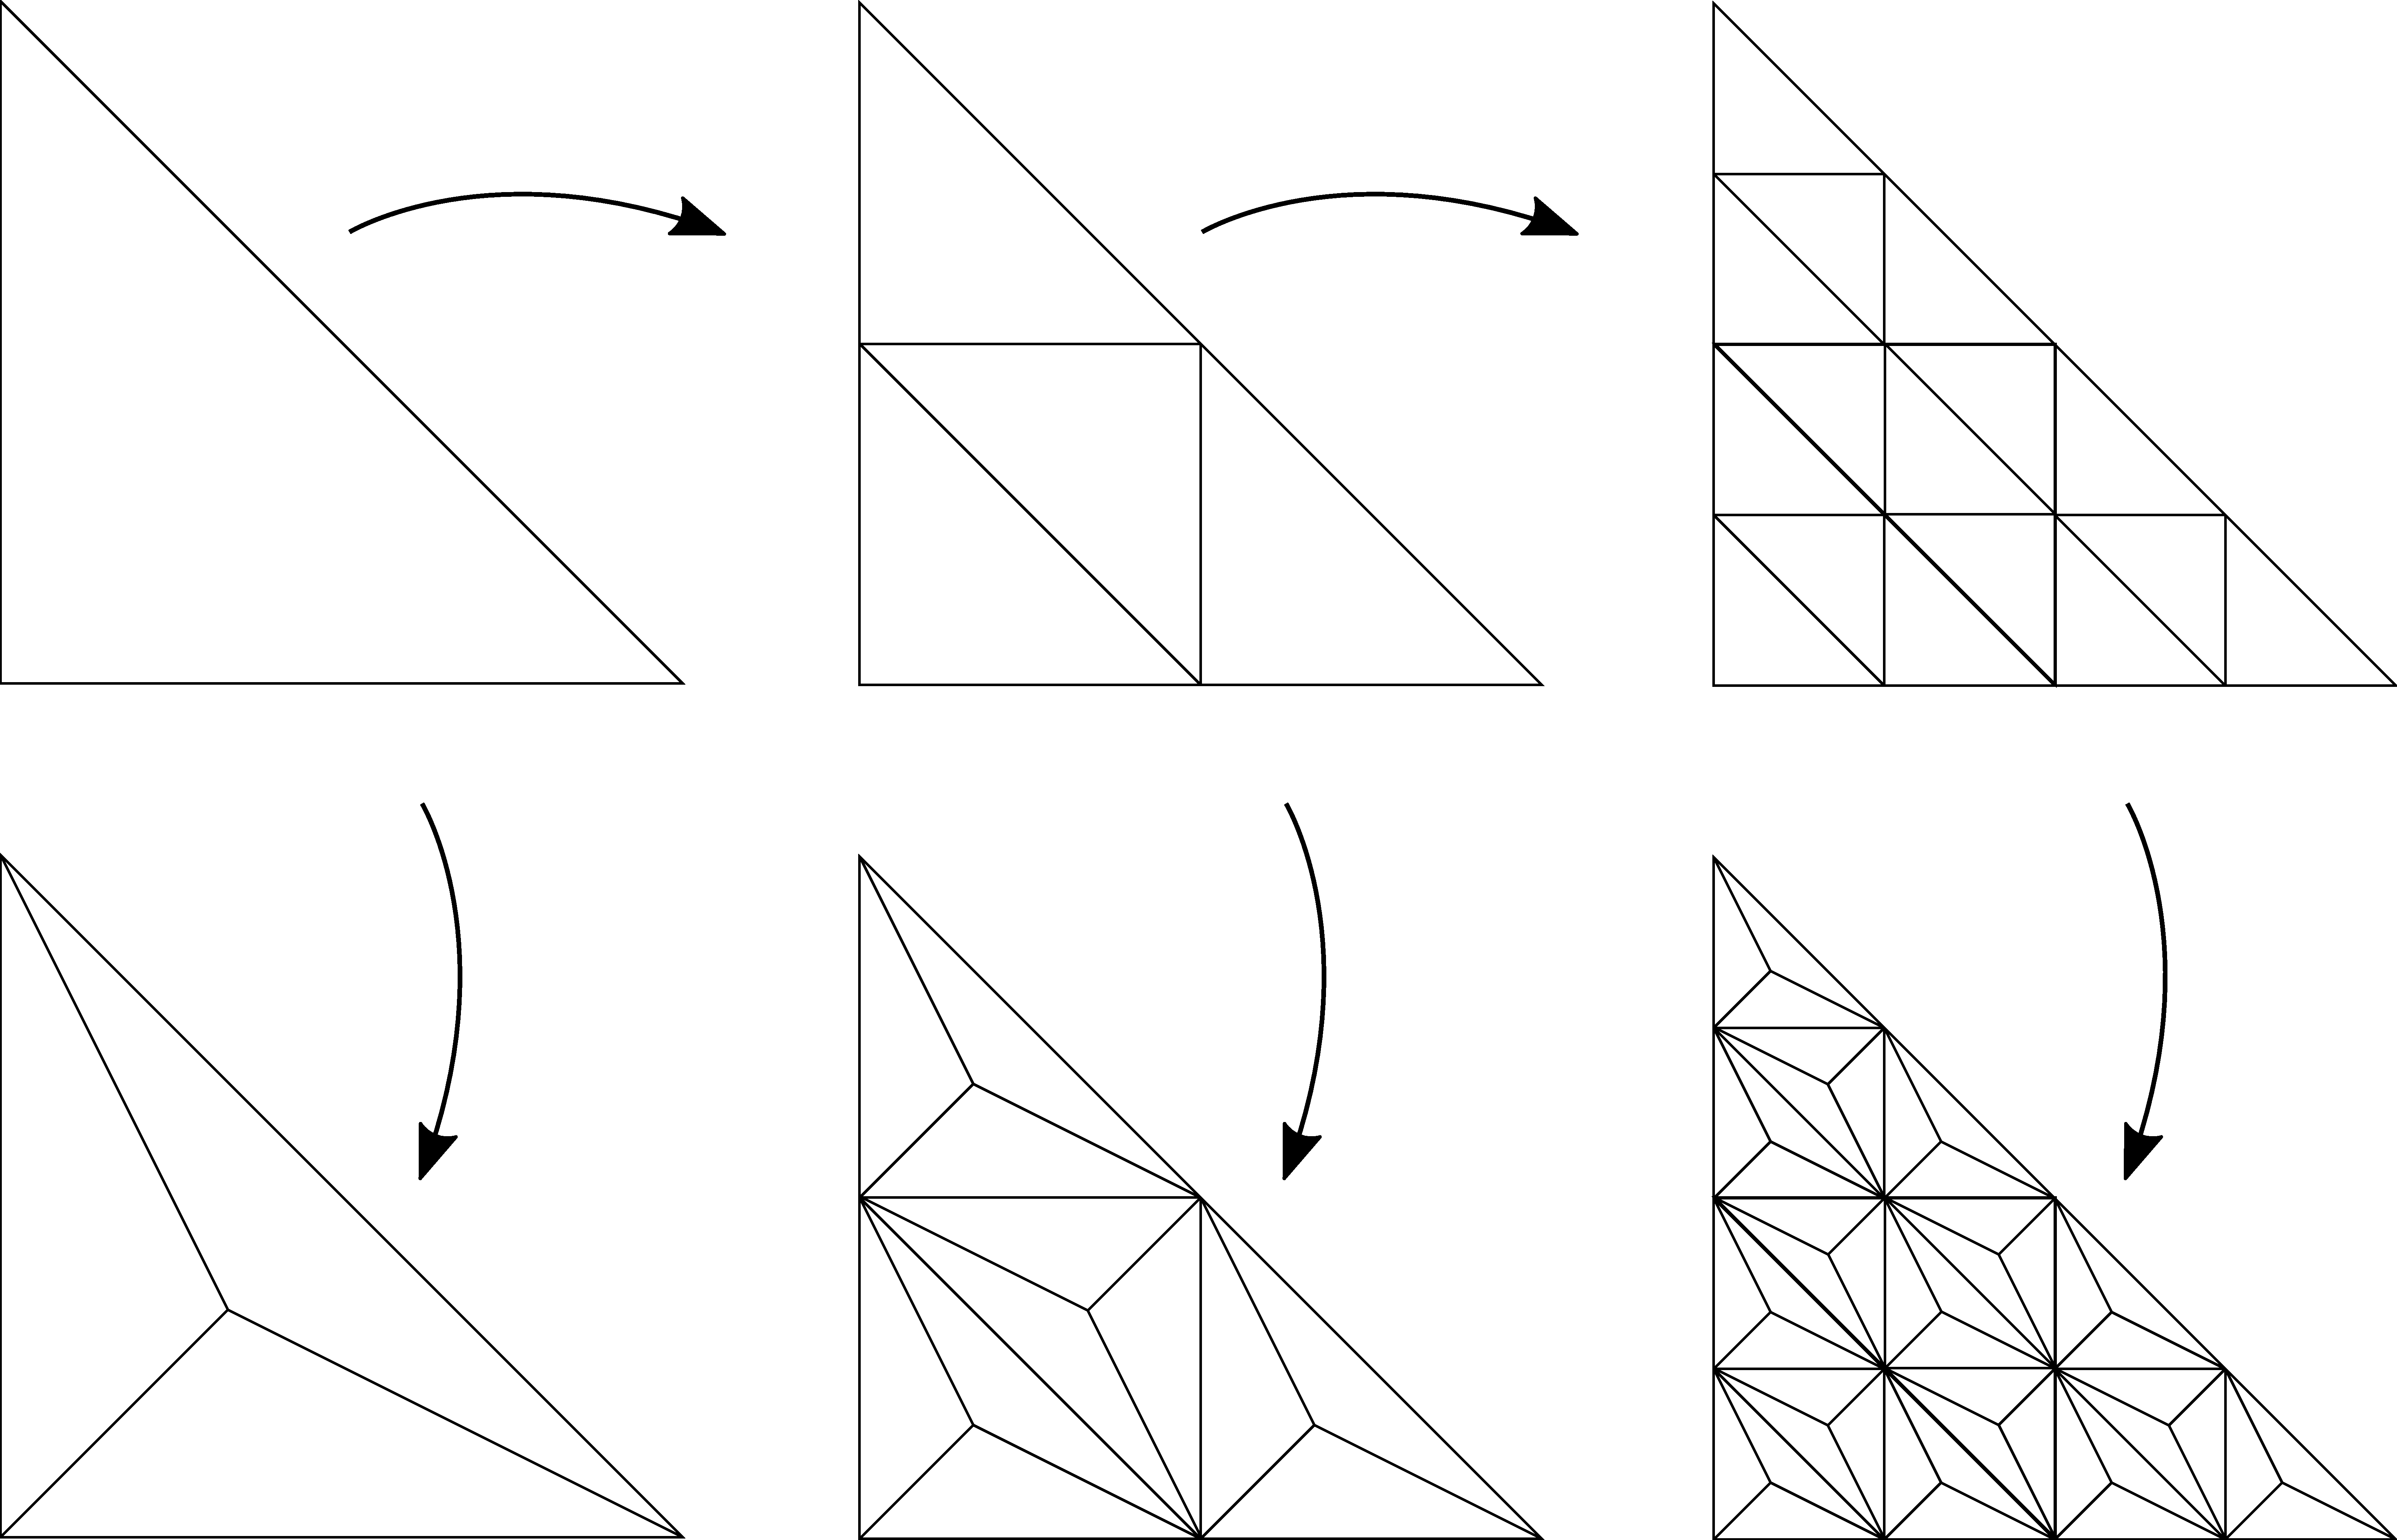
\includegraphics[height=0.6\textheight]{baryhierarchy}
        \end{center}
      \end{block}
    \end{onlyenv}
    \begin{onlyenv}<3>
      \begin{block}{Regular refinement}
        Geometric multigrid. One example of structure-exploitation: Hybrid Hierarchical Grids \parencite{Bergen:2004}.
        \begin{center}
          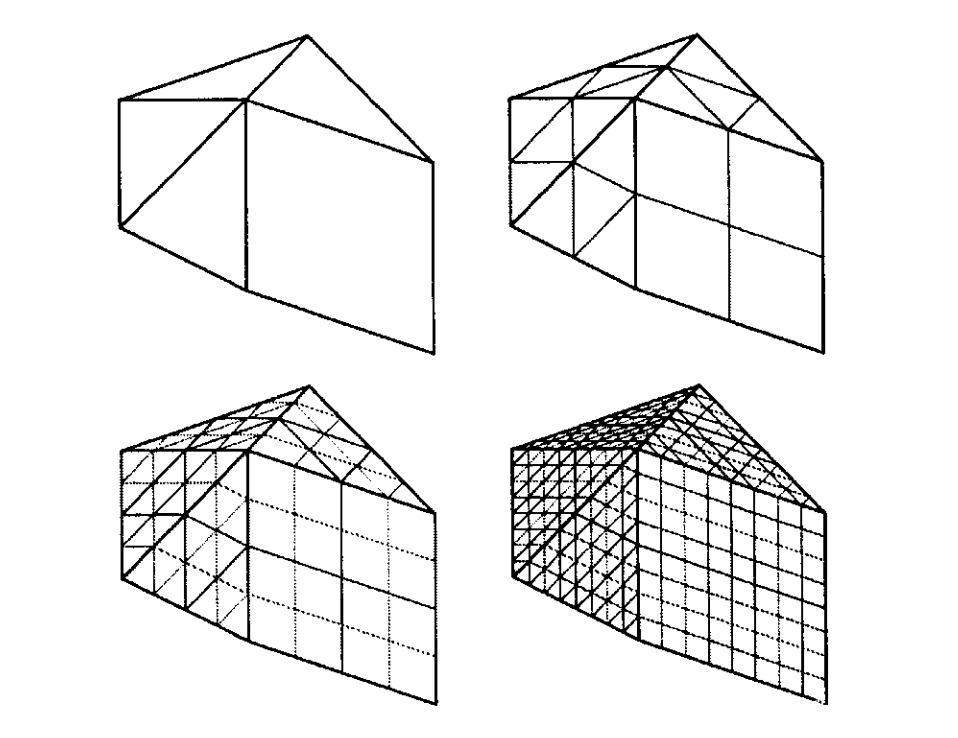
\includegraphics[height=0.6\textheight]{hhg}
        \end{center}
      \end{block}
    \end{onlyenv}
  \end{overlayarea}
\end{frame}
\begin{frame}
  \frametitle{Some motivation: extruded meshes}
  \begin{columns}
    \begin{column}{0.6\textwidth}
      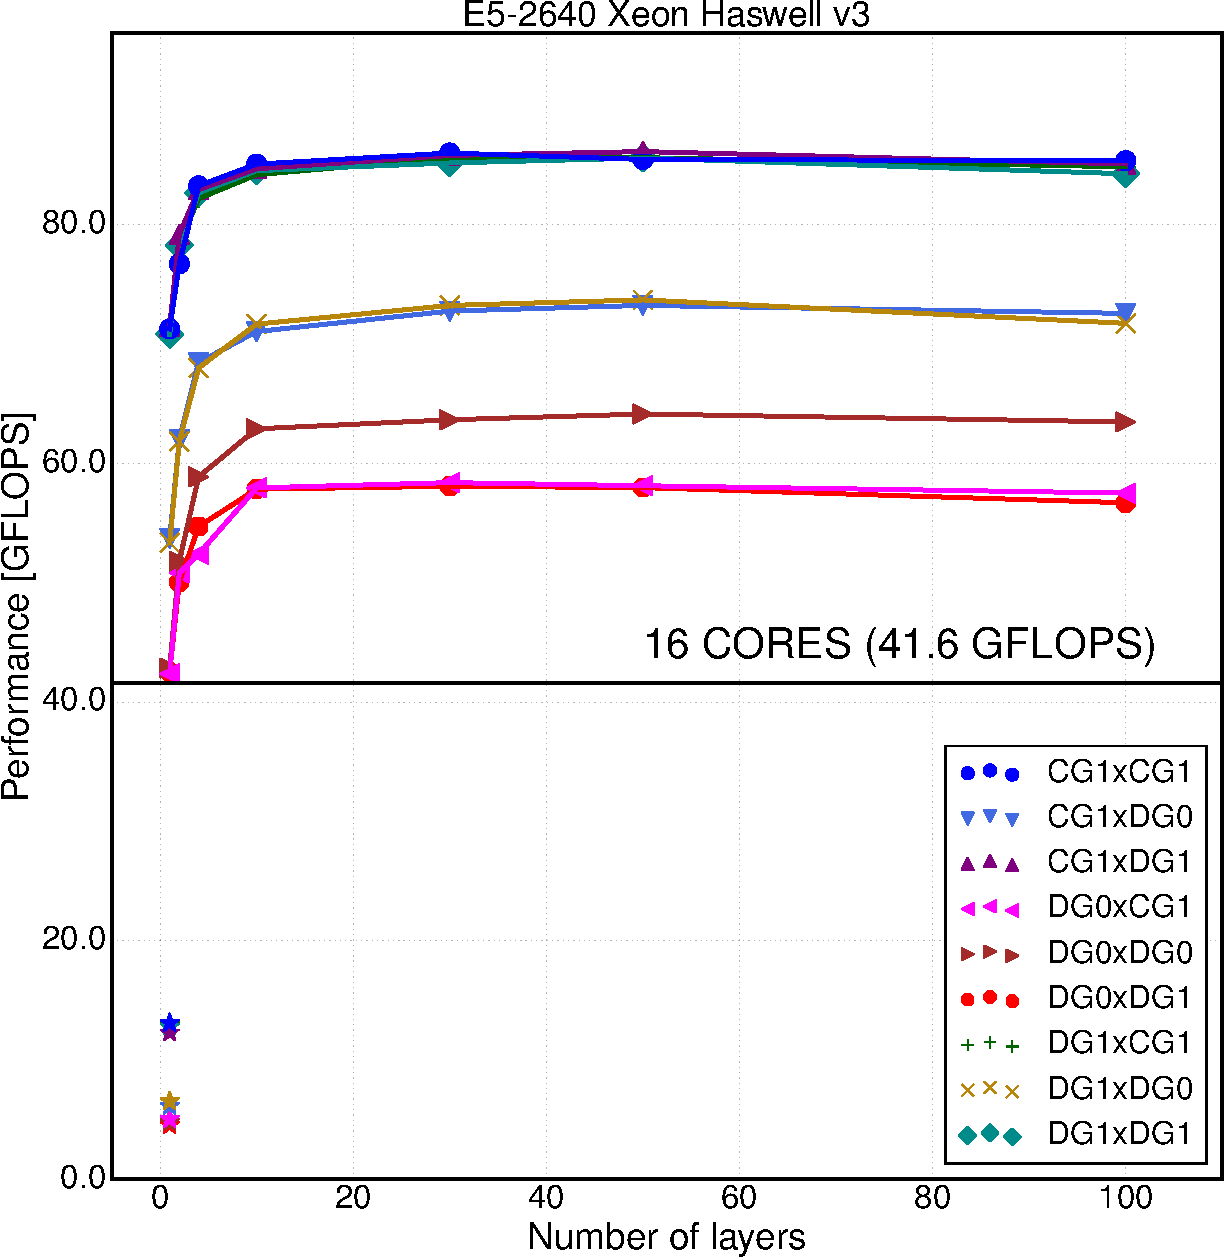
\includegraphics[height=0.7\textheight]{FRHS-32-2}
    \end{column}
    \hspace{-1em}
    \begin{column}{0.45\textwidth}
      \begin{itemize}
      \item Simple residual evaluation: stresses memory subsystem
      \item Increasing number of layers $\Rightarrow$ more structure
      \item Gain $20-40\%$ performance over unstructured case
      \end{itemize}
      \begin{flushright}
        {\footnotesize Bercea et al.~, Geoscientific Model Development
          9(10):3803 (2016), \arxivlink{1604.05937}{cs.MS}}
      \end{flushright}
    \end{column}
  \end{columns}
\end{frame}

\begin{frame}
  \frametitle{Idea: code generation}
  \begin{itemize}
  \item Firedrake exploits structure in extruded meshes, but nothing
    else
  \item Problem: don't want to code the cartesian product of different
    substructure components by hand
  \item Might wish to try different iteration orders, data layout
    
  \item $\Rightarrow$ develop interface for code generation
  \item Challenges: needs to look like a real mesh
  \item $\Rightarrow$ topological queries must work
  \end{itemize}
\end{frame}


\appendix
\begin{frame}
  \frametitle{References}
  \printbibliography[heading=none]
\end{frame}

\end{document}

